% Longueur de référence :
%%%%%%%%%%%%%%%%%%%%%%%%%%%%%%%%%%%%%%%%%%%%%%%%%%%%%%%%%%%%%%%%%%%%%%%%%%%%%%%%%%%%%%%%%%%%%%%%%%%%%%

\chapter{Calcul tensoriel}
\label{chap:ch1}

\section{Notation indicielle}
    \subsection{Définition et exemple}
    Dans le cadre de ce cours, on utilisera les notations indicielles, ou un indice représente un 
    \textit{numéro de composante}. Dans une équation, un indice peut apparaître :
    
    \begin{description}
    \item[1x]; il doit apparaître une fois dans tous les termes de l'équation. C'est un 
    \textit{indice libre}.
    \item[2x]; il représente une sommation. C'est un \textit{indice muet}.
    \end{description}
    Un indice ne peut donc \textbf{jamais} apparaître plus de deux fois dans un même terme.


        \subsubsection{Exemples}
        Le produit scalaire $q = \vec{u}.\vec{n} = u_xn_x + u_yv_y+u_zv_z$ s'écrit en notation
        indicielle:
        \begin{equation}
        q = u_kn_k
        \end{equation}
        
        Le produit vectoriel, $\vec{c} = \vec{a}\times\vec{b}$ s'écrit dès lors :
        \begin{equation}
        c_i = \delta_{ijk}a_jb_k
        \end{equation}
        On voit ici que $i$ est indice libre à gauche et à droite. S'il n'y a pas d'indice libre
        d'un côté, il ne peut \textbf{pas} y en avoir de l'autre côté.
        
        Pour illustrer, voici deux équations \textbf{fausses}
        \begin{enumerate}
        \item $\tau_{kk} = 2\mu a_{kk} + \lambda\delta_{kk}a_{kk}$
        \item $k_{ij} = \lambda_i\delta_{ij}$
        \end{enumerate}
        
        \subsubsection{Remarque}
        Pour les dérivées partielles, on placera l'indice $i$ en indice après la virgule :
        \begin{equation}
        \partial_i \equiv \frac{\partial}{\partial x_i} \equiv (\dots)_{,i}
        \end{equation}
        
        Pour les dérivée temporelle, on utilise l'indice 0 qui n'obéit \textbf{pas} à la
        règle de la notation indicielle ! 
        \begin{equation}
        \partial_0 \equiv \frac{\partial}{\partial t}
        \end{equation}


    \newpage
    \subsection{Rotation des axes}
    \begin{wrapfigure}[7]{l}{3.5cm}
    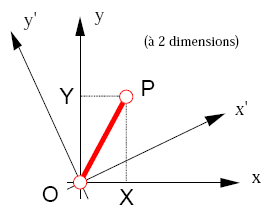
\includegraphics[scale=0.5]{ch1/image1.png}
    \captionof{figure}{Rotation d'axe}
    \end{wrapfigure}
    Considérons les axes $\vec{1_x}, \vec{1_y}$ et $\vec{1_z}$. Définissons $x = OX, y = OY, 
    z = OZ$. Le vecteur $\vec{OP}$ peut s'écrire :
    \begin{equation}
    \vec{OP} = x\vec{1_x} + y\vec{1_y}+z\vec{1_z}
    \end{equation}
    mais ça, c'était avant ! Avec notre superbe notation indicielle, on trouve (où $x = \vec{OP}.
    \vec{1_x}, y = \dots$):
    \begin{equation}
    \vec{OP} = x_i\vec{1_{x_i}}
    \end{equation}
    
    Considérons maintenant un système d'axe $\vec{1_{x'}}, \vec{1_{y'}}$ et $\vec{1_{z'}}$. Notre
    vecteur $x' = \vec{OP}.\vec{1_{x'}}$ avec $\vec{OP} = x\vec{1_x} + y\vec{1_y}+z\vec{1_z}$. On
    trouve donc :
    \begin{equation}
    x' = ( x\vec{1_x} + y\vec{1_y}+z\vec{1_z}).\vec{1_{x'}} = x(\vec{1_x}.\vec{1_{x'}}) + x(\vec{1_y}
    .\vec{1_{y'}}) + x(\vec{1_z}.\vec{1_{z'}})
    \end{equation}
    
    En notant $\cos(x,x') = (\vec{1_x}.\vec{1_{x'}})$\footnote{Le produite scalaire de deux vecteurs
    unitaires donne le cosinus de l'angle entre les deux} \textbf{et} avec $\cos(y',x) = \cos(x,y')$ :
    \begin{equation}
    \left\{\begin{array}{ll}
     x' &=  x\cos(x,x') + y\cos(y,x') + z\cos(z,x')\\
     y' &=  x\cos(x,y') + y\cos(y,y') + z\cos(z,y')\\ 
     z' &=  x\cos(x,z') + y\cos(y,z') + z\cos(z,z')
    \end{array}\right.
    \end{equation}
    
    Ce qui donne, en notation indicielle (c'est dégueu et bien à la fois) :
    \begin{equation}
    x_i' = x_j\cos(x_j,x_i')
    \end{equation}
    et, similairement :
    \begin{equation}
    x_i = x_j'\cos(x_j',x_i)
    \end{equation}
    Il s'agit de \textbf{trois} équations ($i=1,2,3$ avec, dans chacune, une \textbf{somme} sur 
    $j=1,2,3$.\\
    
    Posons $\alpha_{ij} = \cos(x_j',x_i)$ de sorte que $\alpha_{ij} = \alpha_{ji}$ avec $\cos(x_j',
    x_i) = \cos(x_i,x_j')$. \textbf{Ssi} on permute aussi "anciens axes" et "nouveaux axes" (on 
    notera le nouvel axe en majuscule pour éviter toute confusion), on a :
    \begin{equation}
    X_I' = \alpha_{Ij}x_j\ \ \ \text{avec}\ \alpha_{Ij} = \cos(x_I',x_j)
    \end{equation}
    Un exemple d'utilisation est donné slide 13.
    
    \subsection{Le symbole de Kronecker}
    Déjà vu à de maintes et maintes reprises, celui-ci est défini 
    \begin{equation}
    \delta_{ij} = \left\{\begin{array}{ll}
     1&\ si\ i=j  \\
     0&\ si\ i\neq j
    \end{array}\right.
    \end{equation}
    \textbf{Attention} à l'utilisation des règles indicielles : $\delta_{22} = 1$ mais $\delta_{jj}=3$!\\
    
    On peut obtenir celui-ci en notation indicielle de la façon suivante :
    \begin{equation}
    \left.\begin{array}{ll}
    x_j &= \alpha_{Kj}x_K'  \\
    x_K' &= \alpha_{Ki}x_i
    \end{array}\right\} \rightarrow x_j = \alpha_{Kj}\alpha_{Ki}x_i \Rightarrow \delta_{ij} = \alpha_{Kj}
    \alpha_{Ki}
    \end{equation}
    
        \subsubsection{Le symbole de Kronecker $\delta_{ijk}$}
        Il s'agit de la généralisation à trois dimmensions
        \begin{equation}
        \delta_{ijk} = \left\{\begin{array}{ll}
         +1&\ \text{Si $ijk$ est une permutation de 1 2 3}  \\
         -1&  \text{Si $ijk$ est une permutation de 3 2 1}\\
         \ 0& \text{Sinon}
        \end{array}\right.
        \end{equation}
        Cette notation permet d'écrire la $i$ème composante du produit vectoriel $\vec{a}=\vec{b}\times
        \vec{c}$ de la sorte : $a_i = \delta_{ijk}b_jc_k$.
        
        
        
        
        
        
\section{Opérateurs}
    Les différents opérateurs peuvent également s'écrire en notation indicielle. Pour le plus grand 
    bonheur de tous, les voici
    
    \begin{center}
    \begin{tabularx}{10cm}{|X|X|X|X|}
        \hline 
        Opérateur & Notation symbolique& Notation usuelle & Notation indicielle \tabularnewline 
        \hline 
        Gradient & $\overline{grad}\ \phi$ & $\vec{\nabla}\phi$ & $\partial_i \phi = \phi_{,i}$\tabularnewline 
        \hline 
        Divergence & $div\ \vec{v}$ & $(\vec{\nabla}.\vec{v})$ & $\partial_i v_i = v_{i,i}$\tabularnewline
        \hline
        Rotationnel & $\overline{rot}\ \vec{v}$ & $\vec{\nabla}\times \vec{v}$ & $\delta_{ijk}\delta_j v_k$\tabularnewline
        \hline
        Laplacien & $\Delta \phi$ & $(\vec{\nabla}.\vec{\nabla})\phi$ & $\partial_{ii} \phi 
        = \phi_{,ii}$\tabularnewline
        \hline
        \end{tabularx}
    \captionof{table}{Notation des opérateurs en notation hostile}
    \label{tab:comparaison}
    \end{center}
    
\section{Scalaire et vecteur}

    \subsection{Scalaire}
    Il s'agit d'un tenseur d'ordre zéro. Un scalaire est une grandeur mesurée par un nombre 
    \textit{indépendant} du choix des axes de coordonnées (l'énergie cinétique par exemple). Lors d'un
    changement d'axe, la valeur du scalaire n'est pas modifiée.

    \subsection{Vecteur}
    Il s'agit d'un tenseur d'ordre un. Un vecteur est une grandeur mesurée par trois composantes qui
    se transforme selon
    \begin{equation}
    v_K' = \alpha_{Kj}v_j
    \end{equation}
    pour tout changement d'axes de coordonnés (par exemple la vitesse ou la force).

    
        \subsubsection{Amusons-nous avec les vecteurs}
        Soit un vecteur $\vec{v}$ défini par ses composantes\footnote{Je note tout en notation indicielle
        car c'est vraiment un truc de flemmard, et j'aime ça!} :
        \begin{equation}
        \vec{v} = v_i\vec{1_{x_i}}
        \end{equation}
        et soit une direction définie par le vecteur unitaire :
        \begin{equation}
        \vec{1_\mu} = \cos(\mu,x_i)\vec{1_{x_i}}
        \end{equation}
        
        La projection du vecteur $\vec{v}$ sur la direction $\vec{1_\mu}$ s'écrit :
        \begin{equation}
        \vec{v}.\vec{1_\mu} \equiv v^{(\mu)} = v_i\cos(\mu, x_i)
        \end{equation}
     On voit donc qu'un vecteur associe un scalaire $v^{(\mu)}$ à toute direction, par une combinaison
    linéaire des cosinus directeurs de cette direction.\\
    La valeur du scalaire est évidemment indépendante du sytème d'axe ; un tenseur d'ordre 1 associe un 
    tenseur d'ordre 0 à toute direction par ...
        
        
        
\section{Tenseur du second ordre}
    \subsection{Définition}
    En généralisation la définition d'un vecteur, on a : \\
    \textit{Un tenseur associe un vecteur à toute direction, par une combinaison linaire des cosinus
    directeurs de cette direction}
    \begin{equation}
    \overline{T}^{(n)} = \overline{T}_i\cos(n,x_i)
    \end{equation}
    
    Avec l'équation $n_i = \cos(n,x_i)$, l'expression devient :
    \begin{equation}
    \overline{T}^{(n)} = \overline{T}_in_i
    \end{equation}
    
    En exprimant ces vecteurs $\overline{T}_i$ en fonction de leurs composantes :
    \begin{equation}
    \left\{\begin{array}{ll}
     \vec{T_1}&= T_{11} \vec{1_{x_1}}+T_{12} \vec{1_{x_2}}+T_{13} \vec{1_{x_3}}  \\
     \vec{T_1}&= T_{21} \vec{1_{x_1}}+T_{22} \vec{1_{x_2}}+T_{23} \vec{1_{x_3}}  \\
     \vec{T_1}&= T_{31} \vec{1_{x_1}}+T_{32} \vec{1_{x_2}}+T_{33} \vec{1_{x_3}}  
    \end{array}\right.\ \ \ \ \Rightarrow \vec{T_1} = T_{ij}\vec{1_{x_j}}
    \end{equation}

    Un tenseur d'ordre 2 est donc défini par 9 composantes. La composante $j$ de $T^{(n)} =
    T_in_i$ s'écrit $T^{(n)}_j = T_{ij}n_i$ définissant les 9 composantes de $T_{ij}$.
    
    
    \subsection{Changement d'axes}
    Le changement d'axe d'un tenseur d'ordre 2 (du à une rotation) est similaire à celle vue au cours
    de \textit{Mécanique rationnelle II}.
    \begin{equation}
    T'_{PQ} = \alpha_{Pi}\alpha_{Qj}T_{ij}
    \end{equation}
    Un tenseur est ainsi une grandeur mesurée par 9 composantes qui se transforme selon la formule
    énoncée ci-dessus pour tout changement d'axe. Par exemple, le tenseur d'inertie (<3), le tenseur
    des contraintes, des déformations, ...


\section{Autre choses à savoir sur les tenseurs}
    \subsection{Tenseur symétrique et antisymétrique}
        Avant toute chose, énonçons les deux définitions associées :
        \begin{enumerate}
        \item Tenseur symétrique : $T_{ij} = T_{ji}$
        \item Tenseur antisymétrique : $T_{ij} = -T_{ji}$
        \end{enumerate}
        
        \prop{Tout tenseur peut être décomposé en une partie symétrique et une partie 
        antisymétrique
        \begin{equation}
        T_{ij} = \underbrace{\frac{1}{2}(T_{ij}+T_{ji})}_{symétrique} + \underbrace{\frac{1}{2}
        (T_{ij}-T_{ji})}_{antisymétrique}
        \end{equation}
        Afin de s'y retrouver, la partie symétrique sera notée à l'aide de () et la partie 
        antisymétrique à l'aide de [] de la sorte
        \begin{equation}
        T_{ij} = T_{(ij)} + T_{[ij]}
        \end{equation}}\ \\
        
        On démontre aisément que le caractère symétrique ou antisymétrique d'un tenseur est 
        indépendant du système d'axes. Il en découle alors la propriété suivante :\\
        
        \prop{Si $S_{ij}$ est un tenseur symétrique et $A_{ij}$ est un tenseur antisymétrique
        alors
        \begin{equation}
        S_{ij}A_{ij} = 0
        \end{equation}}\ \\
        
        Cela signifie que $T_{11} + T_{22} + T_{33} = 0$. On ne va pas s'attarder la dessus car dans
        le cadre de ce cours cela ne sera que peu utile\footnote{Pareil pour la partie "Des invariants
        d'un tenseur} (comprenez : "passez moi"? :D)
    
    \subsection{Remarque concernant $\alpha_{Pi}$}
    Il faut faire attention à ce qu'est $\alpha_{Pi}$. Celui-ci lie les deux systèmes d'axes mais n'est
    pas défini en tant que tel dans un système : son rôle est de "lier" les axes entres eux mais ce n'
    est \textbf{pas} un tenseur ! 


\section{Théorèmes de Gauss}
    \subsection{Théorème de Gauss 3D}
    Déjà vu en long et en large au cours de \textit{Physique Générale}, le théorème de Gauss s'applique
    dans un volume $V$ limité par une surface fermée $S$\footnote{Suffisamment régulière.}. On l'énonce
    \begin{equation}
    \int_V \partial_i T\dots dV = \oint_S T\dots n_i dS
    \end{equation}
    où $T\dots$ représente un scalaire, vecteur ou tenseur quelconque et $\vec{n}$ la normale unitaire 
    \textbf{extérieure au volume} ! Pour retenir ce théorème, il suffit de savoir que pour passer de
    $dV$ à $dS$ on remplace $\partial_i$ par $n_i$. Comment alors retenir de quel côté est l'un ou
    l'autre ? Il suffit de savoir que l'on ne peut pas avoir de normale à l'intérieur d'un volume :
    $n_i$ doit alors forcément se trouver dans l'intégrale de surface.
    
    \begin{proof}
    Démontrons le théorème pour $i=1$\\
    Je considère un petit rectange $dx_2dx_3$, ce qui me permet de traverser tout mon volume en passant
    par la surface notée $B$ et en sortant par la surface $A$\footnote{Ceci justifie l'intérêt d'avoir
    une forme "suffisament régulière".}. En partant de la définition de l'intégrale de volume :
    \begin{equation}
    \int_V \partial_1 T\dots dV = \iiint \partial_1 T\dots dx_1dx_2dx_3
    \end{equation}
    Ceci est équivalent à
    \begin{equation}
    \iint dx_2dx_2\int_B^A \partial_1\ T\dots dx_1
    \end{equation}
    L'intégrale de la dérivée donne
    \begin{equation}
    \iint (T_A-T_B)dx_2dx_3
    \end{equation}
    Étudions le signe de nos vecteurs normaux
    \begin{equation}
    \left\{\begin{array}{lll}
     (dx_2dx_3)_A & n_1dS_A &\ car\ n_1>0  \\
     (dx_2dx_3)_B & -n_1dS_B &\ car\ n_1<0 
    \end{array}\right.
    \end{equation}
    Notre intégrale devient
    \begin{equation}
    \int_V \partial\ T\dots dV = \iint (T_A-T_B)dx_2dx_3
    \end{equation}
    Définissions (voir schéma ci-dessous) $S'$ la partie de $S$ où $n_1>0$ et $S''$ la partie de $S$ où
    $n_1<0$. On démontre ainsi le théorème
    \begin{equation}
    \iiint \partial_1\ T\dots dx_1dx_2dx_3 = \int_{S'} T\dots n_1 dS' + \int_{S''} T\dots n_1 dS'' =
    \oint_S T\dots n_1 dS
    \end{equation}
    
    \end{proof}
    \begin{center}
    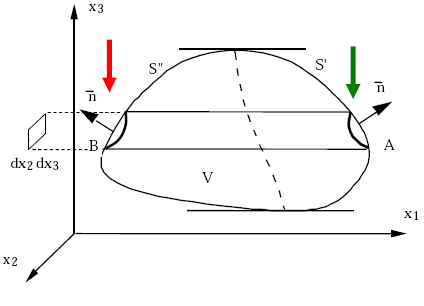
\includegraphics[scale=0.5]{ch1/image2.png}
    \captionof{figure}{Schéma de la démonstration}
    \end{center}
   
   	\textit{NB : Notre $T$ peut valoir trois choses :} 
   	\begin{enumerate}
   	\item \textit{Scalaire}
   	\item \textit{Vectoriel}
   	\item \textit{Tenseur}
   	\end{enumerate}
   	
\section{Notion de débit}
\begin{wrapfigure}[12]{r}{2cm}
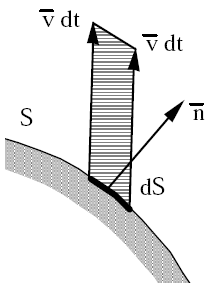
\includegraphics[scale=0.5]{ch1/image3.png}
\captionof{figure}{Notion de débit}
\end{wrapfigure}
Considérons une surface $S$ de normale $\vec n$, la vitesse $\vec{v}$ des points matériels traversant cette
surface ainsi qu'une grandeur $A$ attachée à ces points matériels.\\
Le \textbf{débit de la grandeur $A$} au travers de la surface $S$ est la quantité de cette grandeur 
traversant la surface par unité de temps.\\

En considérant le système après un temps $dt$, les particules se sont déplacées de $\vec{v}dt$. Le
volume de particules ayant traversé la surface $dS$ est le volume hachuré (base * hauteur) sur le
schéma ci-contre : $[\vec{n}.\vec{v}dt]dS$.\\
Le \textbf{débit élémentaire} (volume par unité de temps) de la grandeur $A$ est 
\begin{equation}
dq = A \vec{v}.\vec{n}dS
\end{equation}
où l'on remarque que seule la composante normale contribue au débit.
